\section*{Источники и решения}

\subsection*{Покер: быстрый вопрос}

Этим вопросом меня озадачил Стэн Уэгон, а он нашёл его в книге Аарона Фридланда \cite{18}.

Суть в том, что все \emph{фулл-хаусы} с тремя тузами одинаково сильны, ведь из одной колоды двух таких не набрать.
Однако фулл-хаусы бьются другими комбинациями: любое \emph{каре}, а их 11 штук, и, что важнее для нас, \emph{стрит-флэшами}.
Фулл-хаусы ТТТ99, ТТТ88, ТТТ77, ТТТ66 и ТТТ55 выбивают из колоды максимальное число стрит-флэшей.
Каждый туз выбивает один стрит-флэш, и каждая фоска (карта младшего достоинства) выбивает по пять, то есть всего выбито 13.
Эти фулл-хаусы и являются лучшими.

Если же вы всё равно потребуете ТТТКК, то вас побьют $40 - 6 \z= 34$ стрит-флэшей, или даже $40 - 13 = 37$, если в вашем фулл-хаусе не нашлось всех четырёх мастей.

\subsection*{Восстановление многочлена}

Эту загадку мне подкинул Джо Булер (Рид-колледж), который считает, что она должна быть очень древней.

Как вы наверно уже догадались, достаточно двух запросов:
если $p(1)=n$, то коэффициенты не превышают $n$.
Далее можно взять $x = n + 1$, и записать ответ $(n + 1)$-ичной системе счисления.
Получим все коэффициенты многочлена!

Джо отметил, что если бы разрешалось задавать произвольные числа, то было бы достаточно одного запроса $x = \pi$.
Надо думать, что Оракул найдёт способ выдать значение $p(\pi)$ за конечное время;
если же вместо этого он станет выдавать его десятичное разложение по одной цифре,
то вам придётся понять, когда остановиться.

Хельге Тверберг заметил, что эта задача имеет смысл для многочленов с неотрицательными вещественными коэффициентами.
Чтобы восстановить $p$, сначала спросим $p(1)$; если ответ $0$, то $p = 0$ и задача решена.
В противном случае будем стоить \emph{конечные разности}.
Положим $p_0(x) = p(x)$, и определим рекурсивно последовательность многочленов $p_{i+1}(x) = p_i (x+1) - p_i(x)$.
Отметим, что коэффициенты всех $p_i$-х неотрицательны.
За $k$ вопросов мы можем узнать $p(1),\dots,p(k)$,
а из них вычислить $p_{k-1}(1)$.
Наименьшее $k$ при котором мы получим $0$ это $d+2$, где $d$ --- степень $p$.
Как только мы знаем $d$, любых $d+1$ из $d+2$ имеющихся у нас значений $p$ достаточно, чтобы восстановить многочлен.

\subsection*{Спасите наши души}

На эту игру указал мне аспирант Рэйчел Эссельштейн.
Вместе с множеством других игр, она обсуждается в книге Тома Фергюсона по теории игр \cite{ferguson}.
Этот вариант игры также предлагался на 28-ой Американской математической олимпиаде 1999 годa.

Вопрос кажется туманным, пока не увидишь следующее.
Единственный способ заставить противника походить так, чтобы выиграть на следующем ходу это заставить его ходить внутрь конфигурации S-пусто-пусто-S (мы её будем называть \emph{ямой}).
Например, Тристан может выиграть, если $n = 7$, поставив $S$ в середину, а затем поставив ещё одну $S$ в конце, подальше от ответного хода Изольды.
Теперь у нас есть яма.
После пары ходов на другой стороне, Изольде придётся сходить в яму и проиграть.

То же самое справедливо для любого нечётного $n$ больше $7$ --- Тристану достаточно поставить $S$, в $4$-х или более клеток от обоих концов, построить яму с одной или другой стороны, а затем ждать.

Если $n$ чётное, то у Тристана нет шансов, ведь Изольде не могут достаться одни ямы --- каждый раз на её ходе у неё нечётное число пустых клеток.
Если же $n$ чётное и большое, то Изольда выигрывает, сыграв $S$ далеко от концов и от первого хода Тристана.
Однако, если Тристан начинает с $O$, то Изольде нельзя поставить $S$ рядом, поэтому потребуется дополнительное место.

В случае $n = 14$, если Тристан поставит $O$ на $7$-ю клетку (нумерация от $1$ до $14$), то лучший ответ Изольды --- $S$ на в позиции $11$ (угроза создать яму с $S$ на $14$-й клетке).
В ответ, Тристан может поставить $O$ на $13$-ю или $14$-ю клетку (или $S$ на $12$-ю или $13$-ю). 
Теперь Изольда хотела бы построить яму поставив $S$ на $8$-ю клетку, но ей нельзя, ведь тогда Тристан выиграет, поставив $S$ в $6$-ю позицию.

Таким образом, при $n = 14$ --- ничья;
Изольде нужно, чтобы $n$ было чётным и не менее 16.
В итоге, Тристан выигрывает, если $n$ --- нечётное и не менее $7$,
Изольда --- если $n$ --- чётное и не меньше $16$;
все остальные значения $n$ приводят к ничьей при оптимальной игре.

\subsection*{Пасьянс с шарами}

Эту головоломку (немного в другом виде) можно найти в книге Мартина Гарднера \cite[2.16]{30}, однако там ответ дан без доказательства.
Доказательство из статьи \cite{45}, которое там упомянуто, занимает три страницы и слишком техническое и для Гарднеровской книги, и для моей.

К счастью, есть простой способ понять, что вероятность выигрыша всегда равна $1/2$, независимо от соотношения красных и зелёных шаров в урне.
Ниже приведено рассуждение Серджио Харта из Иерусалимского университета, который и обратил моё внимание на эту задачу.

Иногда в анализе случайного процесса лучше переместить случайность в другое место.
В этой задаче полезно (и допустимо) представить, что перед каждым раундом оставшиеся шары случайно упорядочиваются, и после этого выбираются слева на право.
Тогда в последним раунде, все шары одноцветны.
В предыдущем раунде есть шары обоих цветов, но все красные шары стоят слева, а все зелёные справа, или наоборот.
Независимо от числа шаров каждого цвета на этом этапе (или изначально), эти два порядка равновероятны.
Поскольку первый приводит к выигрышу, а второй к проигрышу, получаем, что вероятность выигрыша равна 1/2.

Серджиу заметил, что этот пасьянс в некотором смысле эквивалентен «Потерянному посадочному талону» \cite[p. 35]{59}.

\subsection*{Пиратская демократия}

Мне напомнил об этой старой загадке аспирант Дартмутского университета Джулио Дженовезе.
Как и многие игры, она решается обратным ходом.
Давайте пронумеруем пиратов от младшего к старшему, и пока будем счиать, что у них всего $n$ монет.
Если дело дойдёт до самого младшего $P_1$, то, он конечно же возьмёт всё золото себе.
(Будем надеяться, что в одиночку он сможет довести корабль к пристани!)

Однако, если дело дошло до $P_1$, то оно дошло и до $P_2$, а
$P_2$, конечно же, оставит себе все монеты и проголосует «за», останется в живых, и возглавит корабль.

Далее, если дело дошло до $P_3$, то он купит голос $P_1$ за одну монету, взяв оставшиеся $n - 1$ себе.
Следовательно, наилучшим вариантом для $P_4$ будет подкупить $P_2$ одной монетой ---
этого достаточно, ведь иначе $P_2$ не получит ничего.

$P_5$ нужны уже два голоса, и он получит их отдав по монете $P_1$ и $P_3$ --- этого достаточно.

Уже видна закономерность, и даже есть утверждение, которое можно пытаться доказывать по индукции:
если осталось нечётное число пиратов, то следует предложить по одной монете каждому оставшемуся нечётному пирату (предполагая, что монет хватит);
если же их чётное число, то следует предложить по одной монете каждому оставшемуся чётному пирату.
По предположению индукции, все получающие монеты пираты проголосуют «за», и теперь уже нечего доказывать.

Ну так что там по поводу капитана?
Для гарантии выживания, ему потребуется 49 монет; дабы предложить по монете всем чётным пиратам ниже 100.

\subsection*{Волшебные рамки}

Эту головоломку предложил Эхуд Фридгут из Еврейского университета; это вариация одной из задач, которая появилась на израильском молодёжном математическом соревновании.
В соревновании рамки были размером $3 \times 3$ и $4 \times 4$.
В этом случае подсчёт вариантов говорит, что всех конфигураций цветов достичь невозможно.
Суть в том, что порядок, в котором располагаются рамки, не имеет значения;
достаточно знать какими способами установки рамок мы воспользовались.
У нас есть $5^2$ способов установки рамки $4 \times 4$
и $6^2$ способов установки рамки $3 \times 3$.
Таким образом, всего $2^{25} \times 2^{36} = 2^{61}$ варианта, этого мало.

Однако, в варианте Фридгута, у нас уже $2^{49} \times 2^{36}$ вариантов, и теоретически этого хватает для получения всех $2^{64}$ конфигураций.
Думаете, теперь получится?

\begin{figure}[ht!]
\centering
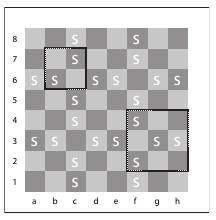
\includegraphics[scale=1]{pics/chess}
\caption{Особые клетки (помечены буквой S) и пара рамок.}
\label{pic:chess1}
\end{figure}

Назовём клетку \emph{особой}, если она находятся в третьей или шестой строке или в третьем или шестом столбце, но не в обоих таких позициях сразу (рис. \ref{pic:chess1}); тогда каждая рамка $2 \times 2$ или $3 \times 3$ покрывает чётное число особых клеток.

Поскольку на доске изначально чётное число чёрных особых клеток, у нас не получится достичь конфигурации, с нечётным  числом чёрных особых клеток.

\subsection*{Больше рамок на меньшей доске}

Эту головоломку подкинул мне Джулио Дженовезе, чей тренер для Олимпиады Патнема, Владимир Чернов, нашёл её в книге «Новые олимпиады по математике» \cite{markova}.

Как и в предыдущей задаче, нужно найти чудесный инвариант.
Однако начнём с совсем неправильной идеи.

Конечно же, достаточно рассматривать только рамки $2 \times 2$, $3 \times 3$ и $5 \times 5$, ведь из них можно составить все остальные.

Как уже было отмечено, стоит проверить, хватит всего того, что разрешается, чтобы сделать всё, что нужно.
Можно думать, что номера на доске это числа по модулю $3$ ($0$, $1$ или $2$, и $2 + 1 = 0$).
Следовательно, нам надо беспокоится о $3^{6^2} = 3^{36}$ возможных конфигурациях.
На каждой клетке доки каждый тип квадрата может быть установлен, не установлен или установлен дважды; установка трижды ничего не даёт.
У нас $5^2$ мест для установки квадрата $2 \times 2$,
$4^2$ для $3 \times 3$
и $2^2$ для $5 \times 5$, так что в общей сложности есть $3^{25} \times 3^{16} \times 3^4 = 3^{45}$ возможных действий, и этого более чем достаточно.
Видимо, на многие из этих действий имеют один эффект.
Так или иначе, пока неясно, можем ли мы получить желаемый результат.

Математически говоря, у нас есть линейное отображение из векторного пространства $\mathbb{Z}_3^{45}$ в векторное пространство $\mathbb{Z}_3^{36}$, и мы хотим узнать всё ли покрывает образ.
(Возможность перехода от конфигурации со всеми нулями к любой произвольной конфигурации эквивалентна обратному.)

Если ответ да, то мы способны перейти от всех $0$ к конфигурации, где все нули, кроме одной единицы в выбранном месте.
Более того, если такое возможно, то задача решена, ведь можно проделать это для каждого местоположения, которому не хватает единицы, и дважды для каждого местоположения, которому не хватает двойки.
Это напоминает поиск решения (с нуля) для кубика Рубика --- нужны операции, которые мало, что меняют.
Например: начнём с двух диагонально смежных квадратов $3 \times 3$ так, что они перекрываются по квадрату $2 \times 2$.
Теперь, если добавить по два подквадрата $2 \times 2$ в каждый угол квадрата $4 \times 4$ и ещё два центральных квадрата, то всё отменится, кроме двух диагонально противоположных углов квадрата $4 \times 4$.
Таким образом, можно увеличить две позиции, одна из которых находится на трёх шагах от другой вдоль диагональной линии.

Однако сложно представить, что возможно изменить одно значение в произвольной позиции.
Давайте поменяем подход.
Если это не так, то есть невозможно получить любую конфигурацию, тогда должен существовать инвариант: некоторое число, связанное с конфигурацией, которое ни один шаг не меняет.
В линейной задаче, подобного рода, этот инвариант сам должен быть линейной функцией.
Это означает, что должно быть два подмножества $A$ и $B$ клеток таких, что если сложить числа в $A$ и прибавить удвоенную сумму чисел в $B$ (в нашей арифметике по модулю $3$ это тоже, что сумма чисел в $A$ минус сумма чисел в $B$), то это даст инвариант.

\begin{figure}[t!]
\centering
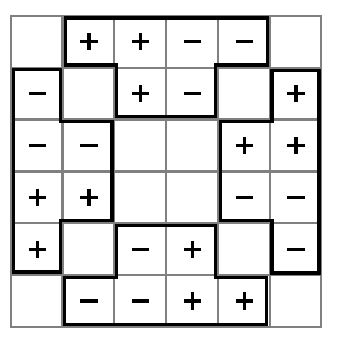
\includegraphics[scale=1]{pics/chess2}
\caption{Множества $A$ и $B$ помеченные знаками $+$ и $-$.}
\label{pic:chess2}
\end{figure}

Построение выше влечёт, что если некоторая позиция находится в $A$, то позиция (всегда есть ровно одна такая) на расстоянии трёх шагов по диагонали должна находиться в $B$, и наоборот.
Исходя из этого наблюдения и зная, что нам нужно в каждом возможной рамке равное число позиций в $A$ и позиций в $B$ (по модулю 3), мы можем найти чудесный узор на рис. \ref{pic:chess2}, в котором точки в $A$ помечены плюсами, а точки в $B$ --- минусами.
И так, мы утверждаем, что сумма значений в позициях $+$, минус сумма значений в позициях $-$, не может измениться.
Отсюда следует, что мы не можем перейти от любой позиции, где это значение не равно $0$, к позиции, в которой все значения равны~$0$.

\subsection*{Простой блеф}

Эта головоломка была предложена Джереми Торпом и Луизой Фуше из Калифорнийского технологического института, но похожие игры были известны и раньше.

Отметим, что имея на руках пику, Луиза всегда выгодно поднимать ставку.
Поэтому у неё есть две \emph{чистые} стратегии:
\begin{itemize}
 \item \textbf{честная} --- поднимать ставку только если есть пика.
 \item \textbf{нахальная} --- всегда поднимать ставку.
\end{itemize}
Если Луиза подняла ставку, то у Джереми есть два варианта ответа:
\begin{itemize}
 \item \textbf{робкий} --- сбросить.
 \item \textbf{смелый} --- проверить.
\end{itemize}

Вероятность вытянуть пику составляет $1/4$.
Значит честная стратегия против робкой даёт Луизе 1 доллар $1/4$ времени, и остальное время 1 доллар выигрывает Джереми.
Ожидаемый выигрыш Джереми составит $1/2$ доллара.
Честная стратегия против смелой даёт Луизе 11 долларов, если у неё пика,
a в среднем приносит ей 2 доллара ($\tfrac14 \times 11 - \tfrac 34 \times 1 = 2$).

Далее, нахальная стратегия против робкой приносит Луизе 1 доллар каждый раз,
в то время как нахальная против смелой обходится ей в $5{,}50$ долларов в среднем ($\tfrac34 \times 11- \tfrac14 \times11 = 5{,}50$).
Если вставить эти числа в матрицу игры $2 \times 2$,
то мы не увидим доминирующей стратегии ни для одного из игроков.
Значит, как и следовало ожидать, придётся использовать вероятностную стратегию.

Из работ Джона фон Неймана (ещё до Джона Нэша) известно, что существует равновесие Нэша для этой игры --- пара стратегий, при которых ни один из игроков не может улучшить свою стратегию, при условии, что другой игрок не меняет свою.
Посмотрим, что это означает для Луизы: если ей не выгодно переходить к честной или нахальной стратегии, то в среднем ей все равно, проверит ли её Джереми или сбросит.

Предположим, что Луиза решила блефовать с вероятностью $p$, если у неё нет пики.
Против робкой стратегии её ожидаемый выигрыш в среднем составит $\tfrac14 \times 1 + p \times \tfrac34 \times 1 - (1 - p) \times \tfrac34 \times 1 =(\tfrac32p - \tfrac12)$ долларов.
Ну а против смелой стратегии, $\tfrac14 \times 11 - p \times \tfrac34 \times 11 - (1 - p) \times \tfrac34 \times 1 \z= (2 - \tfrac{15}2p)$ долларов.

Поскольку Луизе должно быть всё равно, эти две величины должны совпасть, что даёт нам $p = 5/18$.
То есть, Луизе следует блефовать $5$ из $18$ раз, когда у неё нет пики и, конечно, всегда повышать ставку, если пика есть.
Её ожидаемый выигрыш независимо от стратегии Джереми будет
\[\frac32\times\frac5{18}-\frac12=2-\frac{15}2\times\frac5{18}=-\frac1{12}\]
долларов.
То есть в среднем Луиза теряет по $\tfrac1{12}$ доллара за игру.

Немного поразмыслив, можно убедиться, что Луизе выгодно увеличить размер повышения ставки,
однако в среднем она останется в минусе, если конечно играют честно.
Причина в том, что если у неё нет пики, то она не может позволить себе блефовать чаще чем один раз из трёх.
Иначе, с точки зрения Джереми, вероятность того, что у неё была бы пика, составила бы по меньшей мере половину, и поэтому Джереми мог бы просто всегда проверять.
Луиза в лучшем случае выйдет в ноль, при повышениях ставки, и будет терять по доллару без повышений, и значит в среднем будет проигрывать.
Но если $p < 1/3$, то Луиза проигрывает робкой стратегии Джереми;
в этом случае она чаще теряет свою ставку, чем выигрывает.

Здесь важно, что вероятность вытянуть пику составляет одну четверть.
Если бы шансы были чуть выше (скажем, если в колоде нет дамы червей), то большая ставка повернула бы удачу в сторону Луизы.

Вернёмся к исходным 10 долларам.
Можно вычислить стратегию равновесия для Джереми (хотя нам этого и не требуется).
Предположим, что если Луиза повышает ставку, то Джереми проверяет с вероятностью $q$.
Тогда, против луизиной честной стратегии, он получает $\tfrac34 \times 1 - \tfrac14 \times q \times 11 - \tfrac14 \times (1 - q) \times 1 = \tfrac12 - \tfrac52q$ доларов,
а против смелой стратегии $\tfrac34 \times q \times 11 - \tfrac14 \times q \times 11 - (1 - q) \times 1 = \tfrac{13}2q - 1$ долларов.
Полагая, что эти величины равны, получаем $q = \tfrac3{18}$; то есть, Джереми должен проверять только $\tfrac3{18}$ всего времени.
Подстановка $q = \tfrac3{18}$ обратно в выражения даёт Джереми $\tfrac1{12}$ доллара за игру в среднем, как и должно быть, ведь ровно столько теряет Луиза.

\subsection*{Китайский Ним}

Эта игра известна как Китайский ним или как Игра Витоффа;
она появилась в его статье 1907 года \cite{60}.
Игра обсуждается несколько раз в первом и втором томе классической книги Элвина Берлекампа, Джона Конвея и Ричарда  Гая \cite{4}.
Связь с «Надёжными мигалками» приведённой выше была замечена в прекрасной книге Сергея Табачникова \cite{56}.
Однако ни одна из этих книг не приводит вывод стратегии.

Каждая позиция $\{x, y\}$ в игре Алекса и Бет является либо выигрышной, либо проигрышной для игрока, который делает следующий ход, при условии оптимальной игры обоих.
Как и в классическом ниме, проще всего попытаться характеризовать проигрышные позиции, поскольку их меньше.

Как только известны проигрышные позиции, можно вывести правильную стратегию.
Если, например, Алекс находится в выигрышной позиции, то у него должна быть возможность одним ходом перейти к проигрышной позиции для Бет.
Если же Алекс находится в проигрышной позиции, то он может только надеяться на ошибку Бет, или же он по-джентльменски предложит ей сделать первый ход.
Таким образом, стратегия сводится к списку проигрышных позиций.
Но разве здесь нет порочного круга?
Разве нам не нужно знать правильную стратегию, чтобы найти проигрышные позиции?
К счастью, поскольку количество бобов всегда уменьшается, мы можем начать снизу и постепенно подниматься вверх.

Любая позиция с одной пустой кучей или с кучами одинакового размера автоматически является победной.
Не сложно понять, что самая простая проигрышная позиция это $\{1, 2\}$.
После этого можно увидеть, что $\{3, 5\}$, $\{4, 7\}$ и $\{6, 10\}$ также проигрышные.
Но где же закономерность?

Пусть $\{x_1 , y_1\}$, $\{x_2 , y_2\},\dots$ будут проигрышными позициями для первого игрока (не считая $\{0, 0\}$);
мы предполагаем что $x_i < y_i$ и $x_i < x_j$ при $i < j$.
Заметим, что $x_i \ne x_j$ для $i \ne j$, ведь если $x_i = x_j$ то Алекс мог бы сделать ход, от большего из $y_i$ и $y_j$ к меньшему, оставляя Бет в проигрышной позиции --- противоречие.

Немного поразмыслив, приходим к выводу, что если известны все проигрышные позиции от $\{x_1 , y_1\}$ до $\{x_{n-1}, y_{n-1}\}$, то $x_n$ есть наименьшее положительное число, которого нет среди чисел из $\{x_1, \dots , x_{n-1}\} \z\cup \{y_1, \dots , y_{n-1}\}$, а $y_n = x_n + n$.
Заметим, что в этом случае $y_n$ превосходит любое число из $\{x_1, \dots , x_{n-1}\} \cup \{y_1, \dots , y_{n-1}\}$.

Доказательство ведётся индукцией по $n$.
Мы уже знаем, что $x_n$ не может быть среди чисел в $\{x_1, \dots , x_{n-1}\} \cup \{y_1, \dots , y_{n-1}\}$, а также, что не может быть более одного $y_n$, который соответствует этому $x_n$.
Остаётся показать, что позиция $\{x_n, y_n\}$ проигрышная.

Если $\{x_n, y_n\}$ была бы победной, то из неё можно было бы прийти в $\{x_i, y_i\}$ для некоторого $i < n$; но такой позиции нельзя достичь уменьшив меньшую кучу или уменьшив обе кучи на одинаковое число бобов, ведь это сделало бы разницу между двумя кучами $n$ или больше.
Также нельзя её достичь, уменьшив б\'{о}льшую кучу, ведь тогда был бы ещё один игрек для одного икса.
Таким образом, $\{x_n, y_n\}$ проигрышная.

Теперь есть возможность создать список проигрышных позиций любой длины.
Из этого легко вывести стратегию Алекса.
Если он столкнётся с $\{x_i , y_i\}$, он убирает одну или две фишки и надеется на ошибку.
Если он видит $\{x_i , z\}$ для $z > y_i$, он уменьшает $z$ до $y_i$.
Если он видит $\{x_i , z\}$ с $x_i < z < y_i$, то есть разница $d = z - x_i < i$, он берет из обеих куч, чтобы дойти до $\{x_d , y_d\}$ (если $z = y_j$ для некоторого $j < i$, то у него также есть вариант уменьшить $x_i$ до $x_j$).
Если он видит $\{y_i , z\}$ с $y_i \le z$, то может уменьшить $z$ до $x_i$, а может иметь и другие варианты.

Однако потребуется значительное время, чтобы вычислить все проигрышные позиции, скажем до тысячи фишек в каждой куче.
Может можно найти более явное описание проигрышных позиций?

Как мы уже знаем, $x_n$ лежит между $n$ и $2n$ для каждого $n$, ведь $x_n$ стоит сразу после всех $x_i$ и некоторых $y_i$ при $i < n$.
Разумно предположить, что $x_n$ примерно равно $rn$, для некоторого $r$ между $1$ и $2$.
Если это так, то $y_n$ должно быть примерно равным $rn + n = (r + 1)n$.

Если это подтвердится, то $n$ чисел $x_i$ между $1$ и $x_n$ примерно равномерно распределены, и, следовательно, доля $r/(r + 1)$ от их количества будет соответствующих игрекам ниже $x_n$.
Таким образом, у нас около $nr/(r + 1)$ игреков ниже $x_n$, и вместе с $n$ иксами, всего получается $x_n$ чисел; то есть
\[n+n\frac{r}{r+1}=nr,\]
что даёт нам $r + 1 = r^2$ или $r = (1 + \sqrt{5})/2$ --- знакомое \emph{золотое сечение}.

Наверное теперь к вам на ум пришло блестящее наблюдение --- поскольку $r$ иррационально и $\tfrac1r+\tfrac1{r^2}=1$, числа $r$ и $r^2$($= r + 1$) подходят на роль $p$ и $q$ в решении «Надёжных мигалок» из главы 3.
Как мы знаем, любое положительное целое число представлено единственным способом как $\lfloor pm\rfloor$ для некоторого целого $m$, либо как $\lfloor qn\rfloor$ для некоторого целого $n$.

А теперь уже возникает подозрение, что $x_n=\lfloor rn\rfloor$, а $y_n=\lfloor r^2 n\rfloor$.
Конечно же, эти значения обладают желаемым свойствам:
каждое $x_n$ --- наименьшее положительное число, не из $x_1, \dots , x_{n-1}$ или $y_1, \dots, y_{n-1}$, иначе его было бы невозможно получить.
Остаётся, проверить, что $\lfloor r^2 n\rfloor - \lfloor rn\rfloor = n$, но это легко, ведь $r^2 n - rn$ равно целому числу $n$,
поэтому и разница их целых частей обязана быть $n$.
Готово!

Чтоб развлечься давайте найдём ход Алекса из предложенных примеров позиций.
Обратите внимание, что $12 000/r$ чуть меньше $7417$, и $7417r = 12 000.9581\dots$ так что $12 000$ это один из иксов, точнее $x_{7417}$.
Соответствующее значение $y_{7417}$ равно $\lfloor 7417r^2\rfloor = 19 417$, поэтому если в другой куче $20 000$ бобов, Алекс может победить, забрав из неё $20 000 - 19 417 = 583$ боба.
Если же в другой куче всего $19 000$ бобов, то Алекс может выиграть, уменьшив кучи одновременно до $\{x_{7000}, y_{7000}\} = \{11 326, 18 326\}$,
и, поскольку $1900$ случайно оказалось одним из игреков, а именно $y_{2674}$, Алекс также может выиграть, уменьшив $x$-кучу до $x_{2674} = \lfloor 2674r\rfloor = 4326$.

\begin{addedbytheeditors}
\textbf{Редакторам:}
Думаю стоит добавить диаграмму с отмеченными проигрышными позициями скажем до 30--40 --- могу заняться.
\end{addedbytheeditors}
